\chapter{原子核反应}
通过研究核衰变来认识原子核具有相当大的局限性:
\begin{compactitem}
	\item 只涉及不稳定核素向稳定核素的转变,大量稳定核素并不发生衰变;
	\item 是自发过程,不涉及核与核、核与其它粒子的相互作用;
	\item 核衰变仅限于几个MeV的低激发能级,而在高能量范围的核现象会更加丰富多彩……
\end{compactitem} 

\begin{definition}{原子核反应}{nuclear reaction}
	用具有一定能量的粒子(核子、原子核、$\gamma$射线或电子)轰击靶核,使其组成或能量状态发生变化,成为不稳定核素,并放出粒子的过程。
\end{definition}
与自发的衰变不同,核反应是被诱发的过程。

考虑一个典型的核反应
\begin{align}\label{AabB}
	a+\nuc A\to b+\nuc B
\end{align}
其中$a$是入射粒子,$\nuc A$是靶核,$\nuc B$是余核,$b$是出射粒子,这个反应我们可以记作
\[
	\reac AabB,
\]
其中$(a,b)$可以代表一类反应:$(\alpha,\nton),(\nton,\gamma)$等。

实现核反应的粒子来源:
\begin{compactitem}
	\item 放射源:$\alpha,\beta,\gamma,\nton$
	\item 宇宙射线:高能质子、$\nucli4{He}$、中子;
	\item 加速器:质子、中子、重离子、X/$\gamma$射线;
	\item 反应堆:中子、$\gamma$、中微子等。
\end{compactitem}
\section{原子核反应概况}
1919年,Rutherford实现了历史上第一个人工核反应
\[
	\alpha+\nucli{14}N\to\nucli{17}O+\pton.
\]

1932年,John. Cockcroft和Ernest Walton加速质子轰击锂靶,实现了第一个在加速器上实现的核反应
\[
	\pton+\nucli 7{Li}\to\alpha+\alpha.
\]

1934年,Curie夫妇产生第一个人工放射性核素
\begin{gather*}
	\alpha+\nucli{27}{Al}\to\nucli{30}P+\nton,\\
	\nucli{30}P\overset{\SI{2.5}{min}}\semilongrightarrow\nucli{30}{Si}+\elc^++\nu_\elc,\\
	\elc^++\elc^-\to\gamma+\gamma.
\end{gather*}

1932年,Chadwick发现中子
\[
	\alpha+\nucli9{Be}\to\nucli{12}C+\nton.
\]
\paragraph{核反应分类}
按出射粒子分类:
\begin{compactitem}
	\item 核散射:出射粒子和入射粒子是同种粒子;
	
	分为弹性散射$\reac AaaA$和非弹性散射$\reac Aa{a'}{A^\ast}$。
	\item 核转变:出射粒子和入射粒子不同。
	
	若出射粒子有$\gamma$,也叫辐射俘获;若入射粒子有$\gamma$,则称之为光核反应。
\end{compactitem}
按入射粒子分类:中子核反应、带电粒子核反应、光核反应。

按能量分类……一般的原子核物理只涉及低能核反应。
\paragraph{反应道}核反应的入射道和出射道统称为反应道。

各反应道的发生几率是不同的:随入射粒子能量变化,与核反应机制、核结构有关,受守恒条件约束。

\paragraph{核反应中的守恒}电荷、核子数、动量、能量、角动量、宇称守恒。
\section{核反应能和\textit{Q}方程}
核反应\eqref{AabB}中能量守恒
\[
	(m_a+m_{\nuc A})c^2+T_a+T_{\nuc A}=(m_b+m_{\nuc B})c^2+T_b+T_{\nuc B}
\]
核反应过程释放出的能量,称为反应能$Q$
\begin{align}\notag
	Q&=(T_b+T_{\nuc B})-(T_a+T_{\nuc A})\\
	&=(m_a+m_{\nuc A})c^2-(m_b+m_{\nuc B})c^2.
\end{align}
\paragraph{$Q$方程}假设靶核静止$T_{\nuc A}=0$,由动量守恒
\[
	\bm P_a=\bm P_b+\bm P_{\nuc B}.
\]
\begin{center}
	\includegraphics[page=8]{figures/tikz/layouts.pdf}
	\captionof{figure}{核反应动量守恒}
\end{center}
$b$的出射角$\theta$,由余弦定理,不易测量的$T_\nuc B$可被$P_a,P_b,\theta$表示
\[
	P_\nuc B^2=P_a^2+P_b^2-2P_aP_b\cos\theta.
\]
对于低能核反应,用非相对论公式$P^2=2mT$
%Q=\kh{1+\frac{m_b}{m_{\nuc B}}}T_b-\kh{1-\frac{m_a}{m_{\nuc B}}}T_a-\frac{2\sqrt{m_am_bT_aT_b}}{m_{\nuc B}}\cos\theta
\begin{align}\notag
	Q&=T_b+T_{\nuc B}-(T_a+0)\\
	&=\kh{1+\frac{m_b}{m_{\nuc B}}}T_b-\kh{1-\frac{m_a}{m_{\nuc B}}}T_a-\frac{2\sqrt{m_am_bT_aT_b}}{m_{\nuc B}}\cos\theta
\end{align}
进而可得到出射粒子$b$的能量-角度关系
\begin{align}
	T_b=\hkh{\frac{\sqrt{m_am_bT_a}}{m_{\nuc B}+m_b}\cos\theta\pm\sqrt{\kh{\frac{m_{\nuc B}-m_a}{m_{\nuc B}+m_b}+\frac{m_am_b\cos^2\theta}{(m_{\nuc B}+m_b)^2}}T_a+\frac{m_{\nuc B}}{m_{\nuc B}+m_b}Q}}^2.
\end{align}
这就是$Q$方程,\index{$Q$方程}将$T_a,T_b,\theta,Q$四个变量联系起来。

当余核B处于激发态的时候,反应能$Q$也会发生相应的改变。

\section{核反应的阈值}
\paragraph{实验室系与质心系}
入射粒子$a$和靶核A相对于质心C运动的动能之和,称为$a$的相对运动动能$T'$
\begin{align}
	T'=\frac{m_{\nuc A}}{m_a+m_{\nuc A}}T_a
\end{align}
由于A相对实验室L是静止的,$a$在L系下的动能$T_a$,只有一部分构成了内能项$T'$,能够参与核反应,而整个质心系的动能不能参与核反应。

\paragraph{核反应的阈值}
在L系中能够引起核反应的$a$的最低能量$T_\thres$
\begin{align}
	T_\thres=\frac{m_a+m_{\nuc A}}{m_{\nuc A}}\abs Q.
\end{align}
由于质心系要带走动能,$T_\thres$必然比$\abs Q$大。
\paragraph{出射角转换}
出射粒子在L系和C系中速度的关系
\[
	\bm v_b=\bm v'_b+\bm v\CM
\]
\begin{center}
	\includegraphics[page=9]{figures/tikz/layouts.pdf}
	\captionof{figure}{L系和C系速度关系}
\end{center}
由正弦定理、余弦定理等关系
\[
	\begin{cases}
		\frac{v_b'}{\sin\theta\LAB}=\frac{v\CM}{\sin\theta\CM-\sin\theta\LAB}\\
		v_b\cos\theta\LAB=v\CM+v_b'\sin\theta\CM\\
		v_b^2=v\CM^2+v_b'^2+2v\CM v_b'\cos\theta\CM
	\end{cases}
\]
定义
\begin{align}
	\gamma:=\frac{v\CM}{v_b'}.
\end{align}
则
\begin{align}
	\begin{cases}
		\theta\CM=\theta\LAB+\arcsin(\gamma\sin\theta\LAB)\\
		\cos\theta\LAB=\frac{\gamma+\cos\theta\CM}{(1+\gamma^2+2\gamma\cos\theta\CM)^{1/2}}
	\end{cases}
\end{align}
不难用$T'$和$Q$解出$\gamma$
\[
	\gamma^2=\frac{m_am_b}{m_\nuc Am_\nuc B}\frac{m_b+m_\nuc B}{m_a+m_\nuc A}\frac{T'}{T'+Q}
\]
由于$m_a+m_\nuc A\doteq m_b+m_\nuc B$
\begin{align}
	\gamma\doteq\sqrt{\frac{m_am_b}{m_\nuc Am_\nuc B}\frac{T'}{T'+Q}}.
\end{align}
\subparagraph{弹性散射}$Q=0,a=b,\nuc A=\nuc B$,故 
\[
	\gamma=\frac{m_a}{m_\nuc A}.
\]
当$m_\nuc A\gg m_a$时,$\gamma\doteq 0$,$\theta\CM=\theta\LAB$;当$m_\nuc A= m_a$时,$\gamma=1$,$\theta\CM=2\theta\LAB$。
\subparagraph{一般情况}当$\gamma<1$时,$v_b'>v\CM$

当$\theta\CM=\theta\LAB=0$时,$v_b$取最大值$v_{b\max{}}=v_b'+v\CM$;当$\theta\CM=\theta\LAB=\pi$时,$v_b$取最小值$v_{b\min{}}=v_b'-v\CM$。
\begin{center}
	\includegraphics[page=10]{figures/tikz/layouts.pdf}
	\captionof{figure}{$\gamma<1$}
\end{center}

当$\gamma>1$时,$v_b'<v\CM$。会出现圆锥效应:
一个$\theta\LAB$对应两个$\theta\CM$
\[
	\theta_{\mathrm L\max{}}=\arcsin\gamma\iv.
\]
\begin{center}
	\includegraphics[page=11]{figures/tikz/layouts.pdf}
	\captionof{figure}{$\gamma>1$圆锥效应}
\end{center}

\section{核反应截面和产额}
核反应截面$\sigma$的物理意义为一个入射粒子与单位面积上的靶核发生反应的概率。截面的大小与$a,\nuc A$和$T_a$有关。\index{反应截面}

截面的量纲为面积,单位为$\si{barn}$
\begin{align}
	\SI{1}{barn}=\SI{e-24}{cm^2}
\end{align}
与原子核的截面大小相当。

核反应产物的出射可能各向异性,这就会定义微分截面,
\begin{align}
	\sigma(\theta,\phi):=\dv\sigma\Omega(\theta,\phi)
\end{align}
实验测量微分截面,积分可得到总截面。
\[
	\sigma=\int_0^{2\pi}\int_0^\pi\sigma(\theta,\phi)\sin\theta\d\theta\nd\phi=2\pi\int_0^\pi\sigma(\theta)\sin\theta\d\theta.
\]
\paragraph{反应截面转换}出射粒子数不随坐标系的选择而改变
\[
	\sigma\CM(\theta\CM)\d\Omega\CM=\sigma\LAB(\theta\LAB)\d\Omega\LAB
\]
可得
\[
	\sigma\LAB(\theta\LAB)=\frac{(1+\gamma^2+2\gamma\cos\theta\CM)^{3/2}}{1+\gamma\cos\theta\CM}\sigma\CM(\theta\CM).
\]
\paragraph{核反应产额}定义:入射粒子在靶中引起的核反应数$N'$与入射粒子数$I_0$之比,称为核反应产额(yield) $Y$。\index{反应产额}
\begin{align}
	Y:=\frac{N'}{I_0}.
\end{align}
与反应截面$\sigma$和数密度$N$有关。

通过厚度为$D$的靶后,未发生反应的入射粒子数
\[
	-\frac{\d I}{I}=\sigma N\d x,\implies I=I_0\e{-\sigma ND}
\]
故透射率$T=\e{-\sigma ND},$
\begin{align}
	Y=1-\e{-\sigma ND}.
\end{align}
宏观截面($\si{1/cm}$) $\Sigma:=N\sigma$,平均自由程$\lambda=1/\Sigma$,厚靶$D\gg\lambda,Y=1.$

\sectionstar{核反应中的分波分析}
尽管核反应截面的单位$\si{barn}$与原子核截面相近,但是有时候二者也可以差异巨大。入射粒子带来的轨道角动量有不同的组成,可以根据不同的轨道角动量来分析核反应截面。

\paragraph{半经典的分波分析}入射粒子$a$速度$v_a$,相对质心的运动动能
\[
	T'=\frac12\mu v_a^2,\quad \mu:=\frac{m_am_{\nuc A}}{m_a+m_{\nuc A}}.
\]
相对运动动量
\[
	p=\mu v_a=\frac\hbar\barlambda,\quad\lambdabar:=\frac\hbar{p}.
\]
式中$\lambdabar$是约化de Broglie波长。\\
相对运动角动量
\[
	L=\rho p=\frac\rho\barlambda\hbar=\ell\hbar,\implies\rho=\ell\lambdabar,\quad\ell=0,1,\ldots
\]%ħ

$(a,\nuc A)$的碰撞过程,可以被分解为对应于轨道角动量$L=0,\hbar,2\hbar,\ldots$的部分。轨道角动量为$\ell\hbar$的入射粒子与靶核作用的截面为
\[
	S_\ell=\pi(\rho_{\ell+1}^2-\rho_\ell^2)=(2\ell+1)\pi\lambdabar^2.
\]
最大半径$\rho\maxi=R=R_a+R_{\nuc A}$,进而得到反应截面
\begin{align}
	\sigma=\sum_{\ell=0}^{R/\barlambda}(2\ell+1)\pi\lambdabar^2=\pi(R^2+\lambdabar^2),
\end{align}
核的尺寸和粒子的波动性,都对截面有贡献。
\paragraph{量子力学的分波分析}
向$x$方向入射的粒子束可用平面波表示,在有心力场中,球面波分解更合适
\[
	\psi_\i=\e{\i kx}=\e{\i kr\cos\theta}=\sum_{\ell=0}^\infty(2\ell+1)\i^\ell j_\ell(kr)P_\ell(\cos\theta),
\]
波函数远离原子核时,$kr\gg\ell$,
\[
	j_\ell(kr)\doteq\frac{\sin(kr-\pi\ell/2)}{kr}=\i\frac{\e{-\i(kr-\pi\ell/2)}-\e{\i(kr-\pi\ell/2)}}{kr}.
\]
故
\[
	\psi_\i=\frac1{2kr}\sum_{\ell=0}^\infty\i^{\ell+1}(2\ell+1)\fkh{\e{-\i(kr-\pi\ell/2)}-\e{\i(kr-\pi\ell/2)}}P_\ell(\cos\theta).
\]
其中$\e{-\i(kr-\pi\ell/2)}$代表入射球面波,$\e{\i(kr-\pi\ell/2)}$代表出射球面波。
由于原点上有靶核,散射会导致出射波函数的变化,
\[
	\psi=\frac1{2kr}\sum_{\ell=0}^\infty\i^{\ell+1}(2\ell+1)\fkh{\e{-\i(kr-\pi\ell/2)}-\eta_\ell\e{\i(kr-\pi\ell/2)}}P_\ell(\cos\theta).
\]
其中$\eta_\ell$是出射波系数。
故靶核导致的散射
\begin{align}
	\psi_\sca=\psi-\psi_\i=\frac1{2kr}\sum_{\ell=0}^\infty\i^{\ell+1}(2\ell+1)(1-\eta_\ell)\e{\i(kr-\pi\ell/2)}P_\ell(\cos\theta).
\end{align}

散射截面等于散射粒子数比上入射粒子注量率,因此
\[
	\d\sigma_\sca=\frac{j_\sca r^2\d\Omega}{j_\i},
\]
量子力学中
\[
	j=\frac{\hbar}{2m\i}\kh{\psi\cj\pv\psi{r}-\psi\pv{\psi\cj}r}.
\]
以$\ell=0$为例,计算得到
\[
	j_\sca=\frac{\hbar k}m\frac{\abs{1-\eta_0^2}}{4k^2r^2},\quad j_\i=\frac{\hbar k}m.
\]
故
\[
	\dv{\sigma_{\mathrm{sc},0}}\Omega=\frac{\abs{1-\eta_0^2}}{4k^2}=\frac{\barlambda^2}4\abs{1-\eta_0^2},
\]
把所有角动量均考虑进去
\[
	\dv{\sigma_\sca}\Omega=\frac{\barlambda^2}4\abs{\sum_{\ell=0}^\infty\i(2\ell+1)(1-\eta_\ell)P_\ell(\cos\theta)}^2.
\]
对$4\pi$立体角积分得散射截面
\begin{align}
	\sigma_\sca=\pi\lambdabar^2\sum_{\ell=0}^\infty(2\ell+1)\abs{1-\eta_\ell}^2.
\end{align}
对于反应截面,可以认为$a$消失了,类似的推导得出
\[
	\sigma_{\mathrm{r}}=\pi\lambdabar^2\sum_{\ell=0}^\infty(2\ell+1)(1-\abs{\eta_\ell}^2).
\]

\paragraph{低能中子的散射截面}对于低能入射中子,$\ell=0$,波函数简化为 
\[
	u_{\mathrm o}(r)=\frac\i{2k}\kh{\e{-\i kr}-\eta_0\e{\i kr}}.
\]
若入射粒子与核的作用已知,则核内波函数可知,继而可知核边界处的对数导数
\[
	f:=\edg{\frac r{u_{\mathrm o}}\dv{u_{\mathrm o}}r}_{r=R}\implies\eta_0=\frac{f+\i kR}{f-\i kR}\e{-\i2kR}
\]
当$f\to\infty$时,$\eta=\e{-\i2kR}$;当$f\to0$时,$\eta=-\e{-\i2kR}$,慢中子$kR\ll 1$,故 
\begin{align}
	\sigma_{\mathrm{sc},0}=\begin{cases}
		4\pi R^2,&f\to\infty\\
		4\pi\lambdabar^2,&f\to0
	\end{cases}
\end{align}
$4\pi R^2$对应势(形状)弹性散射截面,$4\pi\lambdabar^2$对应共振散射截面。
\paragraph{散射截面vs反应截面}
\begin{center}
	\includegraphics[page=12]{figures/tikz/layouts.pdf}
	\captionof{figure}{散射截面$\sigma_\sca$与反应截面$\sigma_\mathrm r$的允许范围}
\end{center}
允许有纯的散射过程($|\eta_\ell|=1$),但不允许有纯的反应过程。入射道对出射道总是开放的——入射粒子可以沿入射道返回,因此一定存在弹性散射。
\section{核反应机制及核反应模型}
\paragraph{核反应的三阶段描述}Weisskopf将核反应分为了三个阶段:
\begin{compactenum}
	\item \textbf{独立粒子阶段}:
	
	部分入射粒子被吸收,引起核反应;\\
	部分入射粒子被散射,形成弹性散射
	\item \textbf{复合系统阶段}:
	
	入射粒子与靶核交换能量:
	直接作用;形成复合核;中间过程
	\item \textbf{最后阶段}:
	
	复合系统分解为出射粒子和剩余核。
\end{compactenum}
各种截面有关系,间讲义。
\paragraph{复合核模型}核反应被分成相互独立的两个阶段:
\[
	a+\nuc A\to\nuc C^\ast\to\nuc B+b
\]
\begin{compactenum}
	\item 入射粒子射入靶核,与之形成一个复合核,该核处于激发态;
	\item 激发态的复合核可沿入射道弹性散射,也可能开放其它反应道。
\end{compactenum}
复合核的激发能$E^\ast$是相对动能$T'$和结合能$B_{a\nuc A}$的和
\begin{align}
	E^\ast=T'+B_{a\nuc A}=\frac{m_\nuc A}{m_a+m_\nuc A}T_a+B_{a\nuc A}.
\end{align}
复合核发射核子一般需要$\sim\SI{8}{MeV}$的分离能。尽管$E^\ast\sim\SI{20}{MeV}$,但平均到每个核子的能量只有$\SI{0.2}{MeV}$,故复合核的分离需要经过多次碰撞,其寿命$\sim\SIrange{e-18}{e-14}{s}$,对核反应而言,这是较长的时间。

反应截面
\begin{align}
	\sigma_{ab}=\sigma_{\mathrm{CN}}(T_a)W_b(E^\ast),
\end{align}
故复合核如何衰变是与它如何形成无关,只取决于系统现在的能量状态。
\paragraph{共振}只考虑s波,即$\ell=0$的情况,$\eta_0=\e{\i2\delta_0}$
\[
	\sigma_{\mathrm{sc},0}=\pi\lambdabar^2|1-\eta_0|^2=4\pi\lambdabar^2\sin^2\delta_0(T').
\]
当入射中子的能量达到某些值时,$\delta_0(T')=\pi/2$,散射截面达到极大,就出现了共振。

在$\delta_0(T')=\pi/2$处($T'=E_\mathrm R$)做Talyor展开,略去高阶项
\[
	\sigma_{\mathrm{sc},0}=\pi\lambdabar^2\frac{\Gamma^2}{(T'-E_\mathrm R)^2+\Gamma^2/4}.
\]
势弹性散射和共振弹性散射是复数和的关系,因此存在干涉。
\paragraph{慢中子反应}对于慢中子与一个$A>100$的靶核而言,最可几的复合核退激机制是发射$\gamma$射线,$(\nton,\gamma)$反应是个比较慢的过程
\[
	\sigma_{\nton,\gamma}=\pi\lambdabar^2\frac{\Gamma_\nton\Gamma_\gamma}{(T'-E_\mathrm R)^2+\Gamma^2/4}.
\]
由于约化de Broglie波长
\[
	\lambdabar^2=\frac{\hbar^2}{2\mu T'^2}\propto\frac1{v^2}
\]
低能中子进入势阱,$E_\nton\ll V_0$,并不容易
\[
	P\propto k\propto v,\implies\Gamma_\nton\propto v
\]

慢中子的动能,对衰变行为没什么影响,$T'\ll B_{\nton\nuc A}$,故
\[
	E^\ast=\const,\enspace\Gamma_\gamma=\const,
\]

非共振中子,能量的变化对复合核的衰变不再有什么影响了$\Gamma=\Gamma_\nton+\Gamma_\gamma$,$\Gamma_\nton\ll\Gamma_\gamma$,$\Gamma=\const$,故\index{$1/v$规律}
\begin{align}
	\label{slow-neutron}
	\sigma_{\nton,\gamma}\propto\frac1v.
\end{align}
当我们用慢中子来照射靶核时,中子能量的降低将会有助于$(\nton,\gamma)$反应的发生,该反应的截面反比于中子的速度。

这里的讨论是在“中子能量远离共振能量”这个前提下开展的,如果中子的动能碰巧在共振能量附近,则公式中分母的第一项会起作用,使的截面或大或小的偏离$1/v$规律
\paragraph{连续区理论}连续区——$T'$增加,复合核处于高激发态,能级重叠。能级密度加大,能级宽度加大,不再有单能级共振。
\paragraph{总结}截面测量

